\documentclass[12pt, leqno]{article} %% use to set typesize
\usepackage{fancyhdr}
\usepackage[sort&compress]{natbib}
\usepackage[letterpaper=true,colorlinks=true,linkcolor=black]{hyperref}

\usepackage{amsfonts}
\usepackage{amsmath}
\usepackage{amssymb}
\usepackage{color}
\usepackage{tikz}
\usepackage{pgfplots}
\usepackage{listings}
%\usepackage{courier}
%\usepackage[utf8]{inputenc}
%\usepackage[russian]{babel}

\lstdefinelanguage{Julia}%
  {morekeywords={abstract,break,case,catch,const,continue,do,else,elseif,%
      end,export,false,for,function,immutable,import,importall,if,in,%
      macro,module,otherwise,quote,return,switch,true,try,type,typealias,%
      using,while},%
   sensitive=true,%
   alsoother={$},%
   morecomment=[l]\#,%
   morecomment=[n]{\#=}{=\#},%
   morestring=[s]{"}{"},%
   morestring=[m]{'}{'},%
}[keywords,comments,strings]%

\lstset{
  numbers=left,
  basicstyle=\ttfamily\footnotesize,
  numberstyle=\tiny\color{gray},
  stepnumber=1,
  numbersep=10pt,
}

\newcommand{\iu}{\ensuremath{\mathrm{i}}}
\newcommand{\bbR}{\mathbb{R}}
\newcommand{\bbC}{\mathbb{C}}
\newcommand{\calV}{\mathcal{V}}
\newcommand{\calE}{\mathcal{E}}
\newcommand{\calG}{\mathcal{G}}
\newcommand{\calW}{\mathcal{W}}
\newcommand{\calP}{\mathcal{P}}
\newcommand{\macheps}{\epsilon_{\mathrm{mach}}}
\newcommand{\matlab}{\textsc{Matlab}}

\newcommand{\ddiag}{\operatorname{diag}}
\newcommand{\fl}{\operatorname{fl}}
\newcommand{\nnz}{\operatorname{nnz}}
\newcommand{\tr}{\operatorname{tr}}
\renewcommand{\vec}{\operatorname{vec}}

\newcommand{\vertiii}[1]{{\left\vert\kern-0.25ex\left\vert\kern-0.25ex\left\vert #1
    \right\vert\kern-0.25ex\right\vert\kern-0.25ex\right\vert}}
\newcommand{\ip}[2]{\langle #1, #2 \rangle}
\newcommand{\ipx}[2]{\left\langle #1, #2 \right\rangle}
\newcommand{\order}[1]{O( #1 )}

\newcommand{\kron}{\otimes}


\newcommand{\hdr}[1]{
  \pagestyle{fancy}
  \lhead{Bindel, Spring 2020}
  \rhead{Numerical Analysis}
  \fancyfoot{}
  \begin{center}
    {\large{\bf #1}}
  \end{center}
  \lstset{language=Julia,columns=flexible}  
}


\begin{document} 

  \begin{center}
    {\large {\bf Proj 1: Where Are My Glasses?}} \\
    (due: {2020-03-06})
  \end{center}

\begin{figure}
\begin{center}
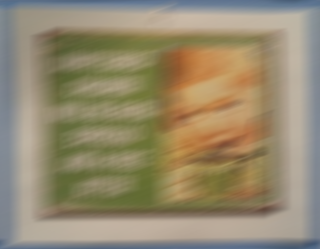
\includegraphics[width=0.5\textwidth]{code/proj1/data/blurry.png}
\end{center}
\caption{A blurred mystery photo taken at the Ithaca SPCA.}
\label{fig1}
\end{figure}

\section{Introduction}

The image in Figure~\ref{fig1} is a blurred version of a picture that
I took at the local SPCA.  As we will see, a naive approach to
de-blurring produces garbage, a characteristic feature of {\em ill-posed}
problems.  In order to reconstruct the image, we need to {\em regularize}
the reconstruction, just as we would regularize an ill-posed least squares
problem.  We will use Tikhonov regularization, as described in class.
However, this involves choosing the value of a
regularization parameter.  Your mission is to investigate the dependence
on the parameter, and to investigate three approaches to
choosing this parameter (mostly) automatically.

You are given the file {\tt blurry.png} (the blurred image shown above)
and several supporting \matlab\ files (Julia and Python versions to be posted).
You are responsible for the following deliverables:
\begin{itemize}
\item Codes to compute ``optimal'' values of the regularization
  parameter $\lambda$ via the discrepancy principle, the L-curve,
  and generalized cross-validation.
\item A report that addresses the questions posed in the rest of this
  prompt.
\end{itemize}
This project is inspired by the project on image deblurring by James
G. Nagy and Dianne P. O'Leary (\href{http://ieeexplore.ieee.org/document/1196312/}{``Image Deblurring: I Can See Clearly
Now''} in {\em Computing in Science and Engineering}; Project: Vol. 5,
No. 3, May/June 2003, pp. 82-85; Solution: Vol. 5, No. 4, July/August
2003).  Other useful references include:
\begin{itemize}
  \item Hansen, Nagy, O'Leary.  \href{http://epubs.siam.org/doi/book/10.1137/1.9780898718874}{\em Deblurring Images: Matrices, Spectra, and Filtering}, SIAM 2006.
  \item Hansen and O'Leary.  \href{http://epubs.siam.org/doi/abs/10.1137/0914086}{``The Use of the L-Curve in the Regularization of Discrete Ill-Posed Problems''} in {\em SIAM J. Sci. Comput.}, Vol 14, No. 6, November 1993.
  \item Golub, Heath, and Wahba.  \href{http://www.stat.wisc.edu/~wahba/ftp1/oldie/golub.heath.wahba.pdf}{``Generalized Cross-Validation as a Method for Choosing a Good Ridge Parameter''} in {\em Technometrics}, Vol. 21, No. 2, May 1979.
  \item Golub and von Matt. \href{https://www.jstor.org/stable/pdf/1390722.pdf}{``Generalized Cross-Validation for Large-Scale Problems''} in {\em Journal of Computational and Graphical Statistics}, Vol. 6, No. 1, March 1997.
  \item Morozov.  \href{https://link.springer.com/book/10.1007%2F978-1-4612-5280-1}{\em Methods for Solving Incorrectly Posed Problems},
  Springer-Verlag, 1984.
\end{itemize}
It should be possible to do this assignment based only on ideas
presented in this prompt and in the lectures.  However,
you are always welcome to use any ideas or code you find in the
literature, including in the references noted above, provided you
give an appropriate citation.

\section{Regularization}

Images in MATLAB are represented as three-dimensional arrays of size
height $\times$ width $\times$ 3, where the three layers represent the
red, green, and blue color intensities at each pixel.  The blurred
image file in Figure~\ref{fig1} has eight-bit color depth, which means
that each of the RGB values is represented as an integer between $0$
and $255$ (inclusive).  Abstractly, we have that for each color plane,
\[
  V^{\mathrm{blur}} = \operatorname{round}(H V^{\mathrm{orig}})
\]
where the round operation represents rounding to the nearest integer
and $H$ is a linear blurring operation.  The matrices
$V \in \bbR^{n \times 3}$ represent images with $n$ pixels and three
colors (though we will always youw the three-index representation
in MATLAB).  Our blurring operation is
a {\em convolution}, which can be diagonalized by a Fourier transform $Z$;
that is,
\[
  H = Z^{*} S Z
\]
where $Z$ is a unitary matrix ($Z^* Z = I$) whose action can be applied
by the two-dimensional fast Fourier transform and $S$ is a diagonal
matrix of eigenvalues.  The matrix $H$ is not symmetric, so the
eigenvalues are complex!

The simplest reconstruction approach is to simply solve
\[
  V^{\mathrm{naive}} \approx H^{-1} V^{\mathrm{blur}}.
\]
which we can do programmatically by
\begin{itemize}
  \item Transforming $V^{\mathrm{blur}}$ into the Fourier basis:
    $\hat{V} = Z V^{\mathrm{blur}}$.
  \item Forming $U = S^{-1} V$ (i.e.~scaling each element of $V$).
  \item Transforming back: $V^{\mathrm{naive}} = Z^* U$.
\end{itemize}
A better approach to deblurring the image is {\em Tikhonov
  regularization}:
\[
  V^{\mathrm{tik}}(\lambda) =
  \operatorname{argmin}_V \|HV-V^{\mathrm{blur}}\|_F^2 + \lambda^2 \|V\|_F^2.
\]
We will now investigate why this approach is better.

\paragraph*{Tasks}
\begin{enumerate}
\item
  Generate a deblurred image by running the following commands
\begin{lstlisting}
  obj = p1setup();
  imnaive = p1tikhonov(obj, 0);
  image(imnaive);
\end{lstlisting}
  Ideally, this naive deblurring approach should reproduce the
  original image.  Does it?  What happens if you set $\lambda = 0.01$,
  i.e.
\begin{lstlisting}
  imtik = p1tikhonov(obj, 0.01);
  image(imtik);
\end{lstlisting}
  Include both images in your report --- you will want to use the
  MATLAB {\tt print} command.

\item
  Look at the code in {\tt p1tikhonov}.  Using your understanding
  of the normal equations and of the eigenvalue decomposition of $H$,
  explain why this code does actually solve the Tikhonov minimization
  problem.

\item
  Because of rounding, the blurred image actually looks like
  \[
    V^{\mathrm{blur}} = HV^{\mathrm{orig}} + E
  \]
  where $E$ is a backward error.  What is the maximum error per pixel
  (assuming no rounding error in applying $H$)?  What is a natural
  bound on $\|E\|_F^2$?

\item
  Using the decomposition $H = Z^* S Z$, what are the singular values
  of $H$?
  The eigenvalues of $H$ are in the {\tt obj.s} vector --- what is the
  smallest singular value?

\item
  Based on the
  error bound on $\|E\|_F^2$ and the value of the smallest singular
  value, provide a bound on $\|V^{\mathrm{orig}}-V^{\mathrm{naive}}\|_F$.
  Compare to $\|V^{\mathrm{blur}}\|_F$, and
  argue that the bad behavior of the naive deblurring approach is
  completely predictable.

\end{enumerate}

\section{Choosing the parameter}

The unsatisfactory feature of Tikhonov regularization is that there
is a free parameter $\lambda$, and so far we have no guidance as to
how to find it.  In the remainder of this project, we consider three
different approaches to finding an ``optimal'' $\lambda$ according
to three different criteria.

\subsection{Morozov's discrepancy principle}

Morozov's discrepancy
principle says roughly that we should choose $\lambda$ so that the
residual
\[
  \rho(\lambda) = \|HV^{\mathrm{tik}}(\lambda) - V^{\mathrm{blur}}\|_F
\]
is about the same size as the difference between $V^{\mathrm{blur}}$
and the ``correct'' right hand side.  Usually this distance is difficult
to estimate (which often makes the discrepancy principle hard to apply
in practice), but in our case we already have a good estimate.

\paragraph*{Tasks}
\begin{enumerate}
\item
  Write a routine to compute $\lambda$ such
  that $\rho(\lambda)$ is approximately $\sqrt{n/4}$ where $n$
  is the number of pixels (this corresponds to assuming the
  rounded-off quantity is uniformly distributed):
  \begin{lstlisting}
  function [lambda] = p1discrepancy(obj, lmin, lmax)
  \end{lstlisting}
  where {\tt lmin} and {\tt lmax} are user-defined lower and upper
  bounds on the value of the regularization parameter $\lambda$.
  If you would like, default values of $10^{-4}$ and $1$ span a good
  range.
  You should feel free to re-use {\tt p1tikhonov} if you would like;
  you may also use {\tt p1applyH}, which applies the blurring operator
  to an image.  You may use \matlab's {\tt fzero} --- or just write a
  bisection routine.
\item
  What is the optimal $\lambda$ by this criterion?
  Show the image for the computed regularization parameter.
\item
  On a log-log scale, plot $\rho(\lambda)$ against $\lambda$ over
  a ``reasonable'' range of values around the recommended
  regularization parameter.  Use a dashed horizontal line to indicate
  $\sqrt{n/4}$, and mark somehow the point on the
  curve associated with the desired value of $\lambda$.  Are there any
  visually distinctive features of the plot that suggest this is
  around the right value?
\end{enumerate}

\subsection{Generalized cross-validation}

The {\em generalized cross-validation criterion} involves minimizing
\[
  G(\lambda) =
  \frac{N \rho(\lambda)^2}
       {\left( \mathrm{tr}(I-H \hat{H}^{\dagger}(\lambda)) \right)^2},
\]
where $\hat{H}^\dagger(\lambda)$ is the solution operator for
the Tikhonov regularized problem ($\hat{H}^\dagger(\lambda) = (H^*H + \lambda^2I)^{-1}H^*$) and $N$ is the number of unknowns
(in this case, three times the number of pixels).  Minimizing $G$ is
easy given the SVD of $H$.  In fact, we know how to compute the SVD
of $H$ in this problem, but in other settings this is not so easy.
So we will seek a different approach.

The troublesome
term is the trace that appears in the denominator, but it turns out
that we can estimate this trace using the fact that if $z$ is any
random vector with independent entries of mean zero and variance one,
then
\[
  \mathrm{tr}(I-H \hat{H}^\dagger(\lambda)) =
  \mathbb{E}\left[ z^T (I-H \hat{H}^\dagger(\lambda)) z \right].
\]
The {\em Hutchinson} estimator uses random probe vectors consisting
of $\pm 1$ entries to estimate the trace of a large matrix, and Golub
and von Matt suggested a procedure that approximates the GCV criterion
with minimization of
\[
  \tilde{G}(\lambda) =
  \frac{Nm^2 \rho(\lambda)^2}
  {\left( \sum_{l=1}^m z_l^T(I-H \hat{H}^{\dagger}(\lambda)) z_l \right)^2},
\]
where each vector $z_l$ is a $\pm 1$ vector drawn using a pseudo-random
number generator.

\paragraph*{Questions/tasks}
\begin{enumerate}
\item
  Show that
  \[
    \frac{d}{d\lambda} \left( I-H \hat{H}^\dagger(\lambda) \right) =
    2\lambda( \hat{H}^\dagger(\lambda) )^* \hat{H}^\dagger(\lambda).
  \]
  From this, you will be able to compute derivatives of $\rho(\lambda)^2$
  and of $z_\ell^T (I-H \hat{H}^\dagger(\lambda)) z_{\ell}$. \\
  {\em Hint:} The expression for differentiating a matrix inverse
  is in your notes!
\item
  For a given set of probe vectors stored in the columns of a matrix
  {\tt Z} in \matlab, write a routine to evaluate $\tilde{G}(\lambda)$
  and the derivative $\tilde{G}'(\lambda)$.  You should need to employ
  multiple factorizations per call:
\begin{lstlisting}
  function [G, dG] = p1gcv(obj, lambda, Z)
\end{lstlisting}
\item
  Using the {\tt p1gcv} function as a building block, write an optimizer
  to minimize the $\tilde{G}$:
\begin{lstlisting}
  function [lambda] = p1gcvopt(obj, lmin, lmax, Z)
\end{lstlisting}
  If the argument {\tt Z} is omitted, form probe vectors with the following
  code fragment
\begin{lstlisting}
  [h,w,~] = size(obj.imblur);
  m = 10;
  Z = sign(rand(h,w,m)-0.5);
\end{lstlisting}
  You should probably make use of the {\tt p1gcv} code from the previous
  question!
\item
  What is the optimal $\lambda$ by this criterion?
  Show the image for the computed regularization parameter.
\item
  On a log-log scale, plot $\tilde{G}(\lambda)$ against $\lambda$ over
  a ``reasonable'' range of values around the recommended
  regularization parameter.  Mark somehow the point on the
  curve associated with the desired value of $\lambda$.  Is
  the curve ``flat'' in the neighborhood of the minimum, or
  is the minimum clearly defined?
\end{enumerate}

\subsection{The L-curve}

The L-curve is a log-log plot of the residual norm ($x$-axis) against
the solution norm ($y$-axis) for varying values of $\lambda$.  It is
named because it tends to look like the letter L.  The vertical part of the L
corresponds to the under-regularized case, where the residual norm
changes negligibly with changes in $\lambda$, but the solution norm
changes dramatically.  The horizontal part corresponds to the
over-regularized case, where small reductions to the solution norm
correspond to increasingly large residuals.  The corner of the L is
the ``sweet spot'' where the two balance each other, and we seek to
find this by finding $\lambda$ where the curvature is maximal.
You are given a function {\tt p1lcurve} that computes a point on the
L-curve (and the curvature) associated with a given $\lambda$;
the function {\tt p1lcurve\_plot} sweeps out the curve, returning
parallel lists of residual norms, solution norms,
logarithmically-spaced values for $\lambda$, and
curvatures $\kappa(\lambda)$.

\paragraph*{Questions/tasks}
\begin{enumerate}
\item
  Draw a (log-log) plot of the L-curve, and a semi-log plot showing
  the curvature as a function of the (log) residual norm.  Is there
  a well-defined corner with a large curvature?
\item
  Write an optimizer to maximize the curvature:
\begin{lstlisting}
  function [lambda] = p1lcurveopt(obj, lmin, lmax)
\end{lstlisting}
  You may use {\tt p1lcurve} to compute $\kappa$, and you may
  use {\tt fminbnd} to do the optimization.
\item
  What is the optimal $\lambda$ by this criterion?
  Show the image for the computed regularization parameter;
  is this a good result?
\end{enumerate}

\section{Notes}

\begin{enumerate}
\item
  The type of very ill-conditioned problems seen here occur frequently
  not only in image reconstruction and inverse problems, but also in
  solving ``first kind'' integral equations that occur in mathematical
  physics.  Integral equations of the second kind tend to be much
  better behaved.
\item
  We have sadly passed on a discussion of the use of iterative solvers
  for treating the large linear systems that arise during the computation
  of the Tikhonov solutions and during the computations involved in
  determining the regularization parameter.
\item
  The types of model selection criteria involved here are useful as well
  for a variety of problems in machine learning --- though we are not
  always so blessed with tricks to make everything efficient!
\item
  As you might gather from our example, though the methods described
  in this project are mostly robust (hence popular) any regularization
  method can be fooled.  There is no substitute for checking the answer
  to see if it looks sensible.
\end{enumerate}

\end{document}
